%!TEX program = pdflatex
\documentclass{beamer}
\usepackage{etex}

\input{./slidespreamble.tex}

\usepackage{tikz}

\usepackage[inline]{asymptote}
\usepackage{attachfile2}
\usepackage{asyfig}
\usepackage{pgfplots}
\pgfplotsset{compat=1.16}



%===========================================================
% Title Info
\title{Scientific Computing for Biologists}
\subtitle{Introduction to matrices} % (optional)

\author{Instructor: Paul M. Magwene}

\date{}



\begin{document}
%===========================================================
\begin{frame}
\titlepage
\end{frame}

% %===========================================================
% \begin{frame}
%   \frametitle{Overview of Lecture}
  
% \begin{itemize}
% 	\item Introduction to Matrices
% 		\begin{itemize}
% 			\item Matrices as collections of vectors
% 			\item Special matrices
% 		\end{itemize}
% 		\item Matrix operations
% 		\begin{itemize}
% 			\item Matrix addition, subtraction
% 			\item Matrix multiplication
% 		  \item Transpose			
% 		  \item More special matrices		  
% 		\end{itemize}		
% 	  \item Matrices concepts		
% 		\item Linear dependence/independence
% 		\item Matrix inverses		
% 		\item Solving simultaneous linear equations
% 	  \item Multiple regression
% \end{itemize}

% \end{frame}
% %===========================================================



%===========================================================
\begin{frame}
  \frametitle{Introduction to Matrices}

\begin{columns}
\begin{column}{5.5cm}

\begin{itemize}
	\item One way to think about a matrix is as a collection of vectors. This is, in essence, what a multivariate data set is.

  \item A matrix which has $n$ rows and $p$ columns will be referred to as a  $n \times p$ matrix.  $n \times p$ is the shape of the matrix.
\end{itemize}

\end{column}

\begin{column}{5cm}

\[
\mathop{A}_{(n \times p)} = \left[ \begin{array}{cccc}

a_{11} & a_{12} & \cdots & a_{1p} \\
a_{21} & a_{22} & \cdots & a_{2p} \\
\vdots & \vdots & \vdots & \vdots \\
a_{n1} & a_{n2} & \cdots & a_{np} \\

\end{array}
\right]
\]

\end{column}

\end{columns}

\end{frame}

%===========================================================


%===========================================================
\begin{frame}
  \frametitle{Special Matrices}

\begin{columns}
\begin{column}{5.25cm}

\begin{itemize}

\item Zero matrix
\[
\mathbf{0} = \left[ \begin{array}{cccc}

0 & 0 & \cdots & 0 \\
0 & 0 & \cdots & 0 \\
\vdots & \vdots & \vdots & \vdots \\
0 & 0 & \cdots & 0 \\

\end{array}
\right]
\]

\item Square matrix

\footnotesize{A matrix whose shape is is $n \times n$}
\[
A = \left[ \begin{array}{cccc}

a_{11} & a_{12} & \cdots & a_{1n} \\
a_{21} & a_{22} & \cdots & a_{2n} \\
\vdots & \vdots & \vdots & \vdots \\
a_{n1} & a_{n2} & \cdots & a_{nn} \\

\end{array}
\right]
\]
\end{itemize}
\end{column}

\begin{column}{5.25cm}
\begin{itemize}
\item Ones matrix
\[
\mathbf{1} = \left[ \begin{array}{cccc}

1 & 1 & \cdots & 1 \\
1 & 1 & \cdots & 1 \\
\vdots & \vdots & \vdots & \vdots \\
1 & 1 & \cdots & 1 \\

\end{array}
\right]
\]

\item Diagonal matrix

\footnotesize{A square matrix where the off-diagonal elements are zero.}

\[
A = \left[ \begin{array}{cccc}

a_{11} & 0 & \cdots & 0 \\
0 & a_{22} & \cdots & 0 \\
\vdots & \vdots & \vdots & \vdots \\
0 & 0 & \cdots & a_{nn} \\

\end{array}
\right]
\]


\end{itemize}
\end{column}

\end{columns}

\end{frame}
%===========================================================


%===========================================================
\begin{frame}
  \frametitle{Scalar Multiplication of a Matrix}


\begin{itemize}
	\item Let $k$ be a scalar and let $A$ be the matrix
	
\[
A = \left[ \begin{array}{cccc}

a_{11} & a_{12} & \cdots & a_{1p} \\
a_{21} & a_{22} & \cdots & a_{2p} \\
\vdots & \vdots & \vdots & \vdots \\
a_{n1} & a_{n2} & \cdots & a_{np} \\

\end{array}
\right]
\]
	

  \item then

\[
kA = \left[ \begin{array}{cccc}

ka_{11} & ka_{12} & \cdots & ka_{1p} \\
ka_{21} & ka_{22} & \cdots & ka_{2p} \\
\vdots & \vdots & \vdots & \vdots \\
ka_{n1} & ka_{n2} & \cdots & ka_{np} \\

\end{array}
\right]
\] 

\end{itemize}

\end{frame}

%===========================================================


%===========================================================
\begin{frame}
  \frametitle{Addition and Subtraction of Matrices}

\begin{itemize}
	\item Let $A$ and $B$ be matrices that have the same shape, $n \times p$:

\[
\begin{array}{cc}
A = \left[ \begin{array}{cccc}

a_{11} & a_{12} & \cdots & a_{1p} \\
a_{21} & a_{22} & \cdots & a_{2p} \\
\vdots & \vdots & \vdots & \vdots \\
a_{n1} & a_{n2} & \cdots & a_{np} \\

\end{array}
\right]

&	

B = \left[ \begin{array}{cccc}

b_{11} & b_{12} & \cdots & b_{1p} \\
b_{21} & b_{22} & \cdots & b_{2p} \\
\vdots & \vdots & \vdots & \vdots \\
b_{n1} & b_{n2} & \cdots & b_{np} \\

\end{array}
\right]
\end{array}
\]	

	
\item then
\[
A + B = \left[ \begin{array}{cccc}
a_{11} + b_{11} & a_{12} + b_{12} & \cdots & a_{1p} + b_{1p} \\
a_{21} + b_{11}& a_{22} + b_{22} & \cdots & a_{2p} + b_{2p}\\
\vdots & \vdots & \vdots & \vdots \\
a_{n1} + b_{n1}& a_{n2} + b_{n2} & \cdots & a_{np} + b_{np}\\
\end{array}
\right]
\]

\[
A - B = A + (-B)
\]

\end{itemize}

\end{frame}

%===========================================================

%===========================================================
\begin{frame}
  \frametitle{Multiplying a Matrix by a Vector}


\begin{itemize}
	\item Let $A$ be a $n \times p$ matrix, and let \Mtx{x} be a $p \times 1$ column vector

\[
\begin{array}{cc}
A = \left[ \begin{array}{cccc}
a_{11} & a_{12} & \cdots & a_{1p} \\
a_{21} & a_{22} & \cdots & a_{2p} \\
\vdots & \vdots & \vdots & \vdots \\
a_{n1} & a_{n2} & \cdots & a_{np} \\

\end{array}
\right]

&	

x = \left[ \begin{array}{c}
x_1 \\ x_2 \\ \vdots \\x_p \\
\end{array}
\right]
\end{array}
\]	

	
\item then
\[
A\Mtx{x} = \left[ \begin{array}{c}
a_{11}x_1 + a_{12}x_2 + \cdots + a_{1p}x_p \\
a_{21}x_1 + a_{22}x_2 + \cdots + a_{2p}x_p \\
\vdots \\
a_{n1}x_1 + a_{n2}x_2 + \cdots + a_{np}x_p \\

\end{array}
\right]
\]

Note that $A\Mtx{x}$ is a vector with shape $n \times 1$. The $i$-the element of $A\Mtx{x}$ is equivalent to the dot product of the $i$-th row vector of $A$ with \Mtx{x}.

\end{itemize}

\end{frame}

%===========================================================

%===========================================================
\begin{frame}
  \frametitle{General Matrix Multiplication}

\begin{itemize}
	\item Let $A$ be a $n \times p$ matrix and $B$ be a $p \times q$ matrix:

\[
\begin{array}{cc}
A = \left[ \begin{array}{cccc}

a_{11} & a_{12} & \cdots & a_{1p} \\
a_{21} & a_{22} & \cdots & a_{2p} \\
\vdots & \vdots & \vdots & \vdots \\
a_{n1} & a_{n2} & \cdots & a_{np} \\

\end{array}
\right]

&	

B = \left[ \begin{array}{cccc}

b_{11} & b_{12} & \cdots & b_{1q} \\
b_{21} & b_{22} & \cdots & b_{2q} \\
\vdots & \vdots & \vdots & \vdots \\
b_{p1} & b_{n2} & \cdots & b_{nq} \\

\end{array}
\right]
\end{array}
\]	

	
\item The product $AB$ is an $n \times q$ matrix whose $(i,j)$-entry is the dot product of the $i$-th row vector of $A$ and the $j$-th column vector of $B$.

\item $A$ and $B$ muse be \emph{conformable} to calculate the product $AB$, i.e. the number of columns in $A$ must be the same as the number of rows in $B$.

\end{itemize}

\end{frame}

%===========================================================

%===========================================================
\begin{frame}
  \frametitle{Matrix Arithmetic Rules}

\begin{enumerate}[i]
	\item $A + B = B + A$
	\item $(A + B) + C = A + (B + C)$ 
	\item $k(A + B) = kA + kB$ 
	\item $(kA)B = k(AB)$
	\item $(AB)C = A(BC)$ (associative)
	\item $A(B+C) = AB + AC$ (distributive)
	\item $(A+B)C = AC + BC$ (distributive)
\end{enumerate}

\begin{Alert}
Matrix multiplication is \emph{\textbf{not}} commutative, i.e. $AB \neq BA$ in general.
\end{Alert}

\begin{center}
\begin{footnotesize}
Be careful when you expand expressions like $(A+B)(A+B)$.
\end{footnotesize}
\end{center}

\end{frame}

%===========================================================


%===========================================================
\begin{frame}
  \frametitle{Matrix Transpose}

\begin{columns}
\begin{column}{5.5cm}

\begin{itemize}
	\item We denote the transpose of a matrix as $A^T$
	
\medskip	

  \item If $A$ is an $n \times p$ matrix, then $A^T$ is a $p \times n$ matrix where $A^T_{ji} = A_{ij}$

  \item Transpose rules:
  \begin{itemize}
  \item $(A^T)^T = A$
  \item $(A + B)^T = A^T + B^T$
  \item $(AB)^T = B^T A^T$
  \end{itemize}

  \item Symmetric matrix-- square matrix, $A$, where $A^T = A$

\end{itemize}

\end{column}

\begin{column}{5cm}

\[
A = \left[ \begin{array}{cccc}

a_{11} & a_{12} & \cdots & a_{1p} \\
a_{21} & a_{22} & \cdots & a_{2p} \\
\vdots & \vdots & \vdots & \vdots \\
a_{n1} & a_{n2} & \cdots & a_{np}
\end{array}
\right]
\]

\[
A^T = \left[ \begin{array}{cccc}

a_{11} & a_{21} & \cdots & a_{n1} \\
a_{12} & a_{22} & \cdots & a_{n2} \\
\vdots & \vdots & \vdots & \vdots \\
a_{1p} & a_{12} & \cdots & a_{np}
\end{array}
\right]
\]

\end{column}
\end{columns}



\end{frame}

%===========================================================


%===========================================================
\begin{frame}
  \frametitle{Identity matrix}

An \emph{identity matrix} is a $p \times p$ matrix with ones on the diagonal and zeros everywhere else.

\[
I = \left[ \begin{array}{cccc}

1 & 0 & \cdots & 0 \\
0 & 1 & \cdots & 0 \\
\vdots & \vdots & \vdots & \vdots \\
0 & 0 & \cdots & 1
\end{array}
\right]
\]

\begin{itemize}
 \item $IA$ = $AI$ = $A$ if $I$ and $A$ are  $n \times p$ matrices
 \item $A = I\Mtx{x}$ is a diagonal matrix where $a_{ii} = x_i$ if $I$ is an $n \times n$ matrix and \Mtx{x} is a $n \times 1$ vector.

\end{itemize}


\end{frame}
%===========================================================


%===========================================================
\begin{frame}
  \frametitle{Matrix Inverse}

\begin{itemize}
\item If $A$ is a \emph{square matrix} and $C$ is a matrix of the same size where $AC = I$ and $CA=I$ than $C$ is the inverse of $A$ and we denote it as \Inv{A}.
\[
A\Inv{A} = \Inv{A}A = I
\]

\item Rules for inverses:

\begin{itemize}
 \item Only square matrices are invertible; but not every square matrix can be inverted
 \item A matrix for which we can find an inverse is called \emph{\textbf{invertible}} (non-singular)
 \item A matrix for which no inverse exists is \emph{\textbf{singular}} (non-invertible)
 \item Any diagonal matrix, $A$, where the $a_{ii}$ are non-zero, is invertible
 \item If $A$ and $B$ are both invertible $p \times p$ matrices than $\Inv{(AB)} = \Inv{B} \Inv{A}$ (note change in order).
\end{itemize}
 
\end{itemize}

% \begin{Highlight}
%   If a matrix is invertible than it's columns form a linearly independent list of vectors!
% \end{Highlight}

\end{frame}
%===========================================================


%===========================================================
\begin{frame}
  \frametitle{}
\begin{center}
\begin{Huge}
{\rmfamily Descriptive statistics as matrix functions}
\end{Huge}
\end{center}
\end{frame}
%===========================================================

%===========================================================

\begin{frame}
  \frametitle{Mean vector and mean matrix}

Assume you have a data set represented as a $n \times p$ matrix, $\Mtx{X}$, with
observations in rows and variables in columns.

\begin{block}{Mean vector}

To calculate a row vector of means, $\Mtx{m} = [\overline{X}_1, \overline{X}_2, \ldots, \overline{X}_p ]$

	\[
	\Mtx{m} = \frac{1}{n} \mathbf{1}^T  \Mtx{X}
	\]

where $\mathbf{1}$ is a $n \times 1$ column vector of ones.

\end{block}

\begin{block}{Matrix of column means}

	\[
	\Mtx{M} = \mathbf{1}\Mtx{m}
	\]

\end{block}

\end{frame}
%===========================================================

%===========================================================
\begin{frame}
	\frametitle{Deviation matrix}

To re-express each value as the deviation from the variable means
(i.e.~each column is a mean centered vector) we calculate a deviation
matrix: 

\[
\Mtx{D} = \Mtx{X} - \Mtx{M}
\]

\end{frame}

%===========================================================


%===========================================================
\begin{frame}
	\frametitle{Covariance and correlation matrices}

\begin{block}{Covariance matrix}
	
\[
\Mtx{S} = \frac{1}{n-1} \Mtx{D}^T \Mtx{D}
\]

\end{block}

\begin{block}{Correlation matrix}

\[
\Mtx{R} = \Mtx{V} \Mtx{S} \Mtx{V}
\]

where \Mtx{V} is a $p \times p$ diagonal matrix where
$\Mtx{V}_{ii} = 1/\sqrt{\Mtx{S}_{ii}}$.
	
\end{block}

\end{frame}
%===========================================================


% %===========================================================
% \begin{frame}
%   \frametitle{Matrix Inverses}

% \begin{itemize}
% \item If $A$ is a \emph{square matrix} and $C$ is a matrix of the same size where $AC = I$ and $CA=I$ than $C$ is the inverse of $A$ and we denote is \Inv{A}.
% \[
% A\Inv{A} = \Inv{A}A = I
% \]

% \item Rules for inverses:

% \begin{itemize}
%  \item Only square matrices are invertible; but not every square matrix can be inverted
%  \item A matrix for which we can find an inverse is called \emph{\textbf{invertible}} (non-singular)
%  \item A matrix for which no inverse exists is \emph{\textbf{singular}} (non-invertible)
%  \item Any diagonal matrix, $A$, where the $a_{ii}$ are non-zero, is invertible
%  \item If $A$ and $B$ are both invertible $p \times p$ matrices than $\Inv{(AB)} = \Inv{B} \Inv{A}$ (note change in order).
% \end{itemize}
 
% \end{itemize}

% \begin{Highlight}
%   If a matrix is invertible than it's columns form a linearly independent list of vectors!
% \end{Highlight}

% \end{frame}
% %===========================================================

%===========================================================
\begin{frame}
  \frametitle{}
\begin{center}
\begin{Huge}
{\rmfamily Simultaneous Linear Equations}
\end{Huge}
\end{center}
\end{frame}
%===========================================================


%===========================================================
\begin{frame}
  \frametitle{Simultaneous Linear Equations}

\begin{itemize}

\item A set of simultaneous linear equations are equations like the following:


\begin{eqnarray*}
2x  +   y   &=&   4 \\
x   -   y   &=&   -1
\end{eqnarray*}

or
 
\begin{eqnarray*}
x + 3y+ 2z & = & 3\\
-x + y + 2z & = & -2\\
2x + 4y -2z & = & 10
\end{eqnarray*}


\end{itemize}





% \item Simultaneous linear equations have either:

% \begin{itemize}
%  \item No solutions
%  \item One solution
%  \item Infinitely many solutions
% \end{itemize}


\end{frame}
%===========================================================

%===========================================================
\begin{frame}[fragile]
  \frametitle{Solving Simultaneous Linear Equations}

Solving a set of simultaneous equations means to find values of the variables where all the equations are true.

\begin{eqnarray*}
2x  +   y   &=&   4 \\
x   -   y   &=&   -1
\end{eqnarray*}

\medskip


\begin{center}
% \begin{tikzpicture}[x=0.3cm, y=0.3cm,domain=-3:5,range=-3:5]
      % \draw[->] (-3,0) -- (5.2,0) node[right] {$x$};
      % \draw[->] (0,-3) -- (0,5.2) node[above] {$y$};
      % \draw[smooth,variable=\x,red]  plot ({\x},{4-2*\x}) node[right] {$2x + y =4$};
      % \draw[smooth,variable=\x,blue] plot ({\x},{1+\x}) node[right] {$x + y = -1$};

\begin{tikzpicture}
\begin{axis}[
    width=0.6\textwidth,
    xlabel={x},
    ylabel={y},
    restrict y to domain=-2:5,
    axis lines=middle, 
    domain=-2:5,
    samples=100,
    xmin=-2, xmax=5,
    ymin=-2, ymax=5,
    enlarge y limits={rel=0.2},
    enlarge x limits={rel=0.2},
]

    \addplot[red] {4-2*x} node[right,pos=1,font=\footnotesize] {$2x + y = 4$};
    \addplot[blue] {1+x} node[left,pos=1,font=\footnotesize] {$x + y = -1$};

\end{axis}      
\end{tikzpicture}

\end{center}


\end{frame}
%===========================================================  

%===========================================================
\begin{frame}
  \frametitle{Solutions to Simultaneous Linear Equations}

Solutions to simultaneous linear equations have either:

\begin{itemize}
 \item No solutions -- inconsistent
 \item One solution -- consistent
 \item Infinitely many solutions -- underdetermined
\end{itemize}

\end{frame}
%===========================================================  



%===========================================================
\begin{frame}
  \frametitle{Matrices and Simultaneous Linear Equations}

\begin{itemize}

\item Matrices can be used to represent and solve simultaneous linear equations. For example,
\begin{eqnarray*}
x_1 + 3x_2 + 2x_3 & = & 3\\
-x_1 + x_2 + 2x_3 & = & -2\\
2x_1 + 4x_2 -2x_3 & = & 10
\end{eqnarray*}

\medskip
Can be represented by the equation $A\Mtx{x} = \Mtx{h}$:

\[
\left[
\begin{array}{ccc}
1 & 3 & 2 \\
-1 & 1 & 2 \\
2 & 4 & -2 \\
\end{array}
\right]
\left[
\begin{array}{c}
x_1 \\ x_2 \\ x_3
\end{array}
\right]
=
\left[
\begin{array}{c}
3 \\ -2 \\ 10
\end{array}
\right]
\]


\item Solve this equation by pre-multiplying both sides of the equation by \Inv{A}.
\begin{eqnarray*}
\Inv{A} A \Mtx{x} & = &\Inv{A} \Mtx{h} \\
\Mtx{x} & = &  \Inv{A} \Mtx{h}
\end{eqnarray*}

\end{itemize}


\end{frame}
%===========================================================

%===========================================================
\begin{frame}
  \frametitle{Simultaneous Equations and Matrix Inverses}

\begin{itemize}
\item $A\Mtx{x} = \Mtx{h}$ has a unique solution iff $A$ is invertible.

\item If $A$ is a singular matrix than $A\Mtx{x} = \Mtx{h}$ either has no solution or infinitely many solutions.

\end{itemize}

\end{frame}
%===========================================================



%===========================================================
\begin{frame}
  \frametitle{}
\begin{center}
\begin{Huge}
{\rmfamily Matrix Concepts}
\end{Huge}
\end{center}
\end{frame}
%===========================================================


% %===========================================================
% \begin{frame}
%   \frametitle{Linear Dependence and Simultaneous Linear Equations}

% Recall that sets of simultaneous linear equations have either:

% \begin{itemize}
%  \item No solutions
%  \item One solution
%  \item Infinitely many solutions
% \end{itemize}

% If the linear

% \end{frame}
% %===========================================================  




%===========================================================
\begin{frame}
  \frametitle{Space Spanned by a List of Vectors}


\begin{block}{Definition}

Let $X$ be a finite list of $n$-vectors. The \textbf{space spanned} by $X$ is the set of all vectors that can be written as linear combinations of the vectors in $X$.
\medskip

% A space spanned includes the zero vector and is closed under addition and multiplication by a scalar.

\end{block}
\bigskip

Remember that a \emph{linear combination} of vectors is an equation of the form $z = b_1 \Mtx{x}_1 + b_2 \Mtx{x}_2 + \cdots + b_p \Mtx{x}_p$

\end{frame}

%===========================================================

%===========================================================
\begin{frame}
  \frametitle{Linear dependence and independence}

\begin{itemize}
% \item You'll remember that a \emph{linear combination} of vectors is an equation of the form $z = b_1 \Mtx{x}_1 + b_2 \Mtx{x}_2 + \cdots + b_p \Mtx{x}_p$

\item A list of vectors, $\Mtx{x}_1, \Mtx{x}_2, ..., \Mtx{x}_p$ , is said the be \emph{\textbf{linearly dependent}} if there is a non-trivial linear combination of them which is  equal to the zero vector.
\[
 b_1 \Mtx{x}_1 + b_2 \Mtx{x}_2 + \cdots + b_p \Mtx{x}_p = 0
\]

\item A list of vectors that are not linearly dependent are said to be \emph{\textbf{linearly independent}} 

\end{itemize}

\end{frame}
%===========================================================





%===========================================================
\begin{frame}
  \frametitle{Subspaces}

$\RealN$  denotes the seat of real $n$-vectors - the set of all $n \times 1$ matrices with entries from the set $\Real$ of real numbers.
\medskip

\begin{block}{Definition}

A \textbf{subspace} of $\Real^n$ is a subset S of $\Real^n$ with the following properties:
\begin{enumerate}
	\item $\Mtx{0} \in S$
	\item If $\Mtx{u} \in S$ then $k\Mtx{u} \in S$ for all real numbers $k$
	\item If $\Mtx{u} \in S$ and  $\Mtx{v} \in S$ then $\Mtx{u} + \Mtx{v} \in S$
\end{enumerate}

\end{block}

Examples of subspaces of $\Real^n$:
\begin{itemize}
	\item any space spanned by a list of vectors in $\Real^n$
	\item the set of all solutions to an equation $A\Mtx{x} = \Mtx{0}$ where $A$ is a $p \times n$ matrix, for any number p.
\end{itemize}

\end{frame}
%===========================================================

%===========================================================
\begin{frame}
  \frametitle{Basis}

Let $S$ be a subspace of \RealN.  Then there is a finite list, $X$, of vectors from $S$ such that $S$ is the space spanned by $X$.
\medskip

Let $S$ be a subspace of $\RealN$ spanned by the list $(u_1, u_2, \ldots, u_n)$. Then there is a linearly independent sublist of $(u_1, u_2, \ldots, u_n)$ that also spans $S$.
\medskip

\begin{block}{Definition}
A list $X$ is a \textbf{basis} for $S$ if:
\begin{itemize}
\item $X$ is linearly independent
\item $S$ is the subspace spanned by $X$
\end{itemize}
\end{block}

\end{frame}
%===========================================================

%===========================================================
\begin{frame}
  \frametitle{Dimension}
Let $S$ be a subspace of \RealN.
\bigskip

\begin{block}{Definition}
The \textbf{dimension} of $S$ is the number of elements in a basis for $S$.
\end{block}

\end{frame}
%===========================================================


%===========================================================
\begin{frame}
  \frametitle{Rank of a Matrix}
Let $A$ by an $n \times p$ matrix.
\bigskip

\begin{block}{Definition}
The \textbf{rank} of $A$ is equal to the dimension of the row or column space of $A$.

\end{block}
\bigskip
Where the row space of $A$ is the space spanned by the row vectors of $A$ and the column space of $A$ is defined similarly.

\end{frame}
%===========================================================




\end{document}



%===========================================================
\begin{frame}
  \frametitle{}
\begin{center}
\begin{Huge}
{\rmfamily Multiple regression}
\end{Huge}
\end{center}
\end{frame}
%===========================================================


%===========================================================
\begin{frame}[fragile]
  \frametitle{Variable space view of multiple regression}

\begin{center}
\includegraphics[height=2.5in]{fig-regression-variable-space.pdf}
\end{center}


\end{frame}
%===========================================================


%===========================================================
\begin{frame}
  \frametitle{Subject Space Geometry of Multiple Regression}

\begin{center}
%\asyinclude[height=2.5in,inline=true]{fig-multiregr.asy}
\includegraphics[height=2.5in]{fig-multiregr.pdf}

\end{center}
\end{frame}

%===========================================================
\begin{frame}
  \frametitle{Multiple Regression}

Let $\Mtx{y}$ be a vector of values for the outcome variable. Let $\Mtx{X}_i$ be explanatory variables.

\bigskip

The regression model is:

$$
\Mtx{y} = \widehat{\Mtx{y}} + \Mtx{e}
$$

where

$$
\widehat{\Mtx{y}} = a\Mtx{1} + b_1\Mtx{X}_1 + b_2\Mtx{X}_2 + \cdots + b_p\Mtx{X}_p
$$

\bigskip

Note that $\widehat{\Mtx{y}}$ is a linear combination of the column vectors of $\Mtx{X}_i$.



\end{frame}
%===========================================================

%===========================================================
\begin{frame}
  \frametitle{Matrix representation of multiple regression}


$$
\Mtx{y} = \widehat{\Mtx{y}} + \Mtx{e}
$$
looks like:
$$
\left[ \begin{array}{c}
y_1 \\ y_2 \\ \vdots \\y_n \\
\end{array}
\right] = 
\left[ \begin{array}{c}
\hat{y}_1 \\ \hat{y}_2 \\ \vdots \\\hat{y}_n \\
\end{array}
\right]+
\left[ \begin{array}{c}
e_1 \\ e_2 \\ \vdots \\e_n \\
\end{array}
\right]
$$

\medskip

We can solve for $\widehat{\Mtx{y}}$ as:
%
$$
\widehat{\Mtx{y}} = \Mtx{X}\Mtx{b}
$$

where
%
$$
\Mtx{X} = \left[ \begin{array}{ccccc}
1 & x_{11} & x_{12} & \cdots & x_{1p} \\
1 & x_{21} & x_{22} & \cdots & x_{2p} \\
\vdots & \vdots & \vdots & \vdots & \vdots \\
1 & x_{n1} & x_{n2} & \cdots & x_{np} \\
\end{array}
\right]
\;
;
\;
\Mtx{b} = \left[ \begin{array}{c}
a \\ b_1 \\ b_2 \\ \vdots \\ b_p \\
\end{array}
\right]
$$

\end{frame}
%===========================================================
\begin{frame}
  \frametitle{Finding the Multiple Regression Coefficients}

How do we solve for \Mtx{b} in $\widehat{\Mtx{y}} = \Mtx{X}\Mtx{b}$?

\bigskip

Estimate \Mtx{b} as:
$$
\Mtx{b} = (\Mtx{X}^T \Mtx{X})^{-1}\Mtx{X}^T\Mtx{y}
$$

\bigskip

Compare this to our formula for estimating the coefficient $b$ in the bivariate regression of $\Vec{y}$ on a single variable $\Vec{x}$:
$$
b = \frac{\Vec{x} \cdot \Vec{y}}{\Vec{x} \cdot \Vec{x}}
$$


\end{frame}
%===========================================================
\begin{frame}
  \frametitle{Multiple Regression ``Loadings''}


In addition to the regression coefficients, the \textbf{regression ``loadings''} -- the cosine of the angle between vectors that represent the explanatory variables and the prediction vector -- are also very useful for interpretting the regression model.

\begin{center}
%\asyinclude[viewportwidth=0.3\textwidth,height=1.5in,keepAspect=true,inline=true]{fig-multiregr-loadings.asy}
\includegraphics[height=1.5in]{fig-multiregr-loadings.pdf}
\end{center}

Individual loadings can be calculated as:
        \[
        \cos \theta_{\vec{x_j},\vec{\widehat{y}}} = \frac{\vec{x_j} \cdot \vec{\widehat{y}}}{|\vec{x_j}||\vec{\widehat{y}}|}
        \]


\end{frame}
%===========================================================


%===========================================================
\begin{frame}
  \frametitle{Multiple Regression, Goodness of fit}

As with bivariate regression, we quantify goodness of of the regression model using the coefficient of determination.

\bigskip

The `multiple correlation coefficient' $R$ is defined as:

$$
R = \cos \theta_{y,\widehat{y}} = \frac{|\widehat{\Mtx{y}}|}{|\Mtx{y}|}
$$

\bigskip

and the coefficient of determination, $R^2$ is:

$$
R^2 = \frac{|\widehat{\Mtx{y}}|^2}{|\Mtx{y}|^2}
$$

\end{frame}
%===========================================================

%===========================================================
\begin{frame}
  \frametitle{Multiple regression: Cautions and Tips}


\begin{itemize}
    \item Comparing the size of regression coefficients only makes sense if all the predictor variables have the same scale
    \item The predictor variables  (columns of $\Mtx{X}$) must be linearly independent; when they're not the variables are \textbf{multicollinear}
    \item Predictor variables that are \textbf{nearly multicollinear} are, perhaps, even more difficult to deal with
\end{itemize}

\end{frame}

%===========================================================

\begin{frame}
  \frametitle{Why is near multicollinearity of the predictors a problem?}

\begin{figure}
\begin{center}
%\subcaptionbox{Non-collinear predictors}{\asyinclude[height=1.35in,keepAspect=true]{fig-regr-noncolinear.asy}}
\subcaptionbox{Non-collinear predictors}{\includegraphics[height=1.25in]{fig-regr-noncolinear.pdf}}
%\subcaptionbox{Nearly collinear predictors}{\asyinclude[height=1.35in,keepAspect=true]{fig-regr-colinear.asy}}
\subcaptionbox{Non-collinear predictors}{\includegraphics[height=1.25in]{fig-regr-colinear.pdf}}
\end{center}
\caption{When predictors are nearly collinear, small differences in the vectors can result in large differences in the estimated regression.}
\end{figure}


\end{frame}

%===========================================================

\begin{frame}
  \frametitle{What can I do if my predictors are (nearly) collinear?}

\begin{itemize}
    \item Drop some of the linearly dependent sets of predictors.
    \item Replace the linearly dependent predictors with a combined variable.
    \item Define orthogonal predictors, via linear combinations of the original variables (PC regression approach)
    \item `Tweak' the predictor variables so that they're no longer multicollinear (Ridge regression).
\end{itemize}


\end{frame}
%===========================================================


%===========================================================
\begin{frame}
  \frametitle{}
\begin{center}
\begin{Huge}
{\rmfamily Linear transformations}
\end{Huge}
\end{center}
\end{frame}
%===========================================================

%===========================================================
\begin{frame}
  \frametitle{Matrices as Linear Transformations}

\begin{itemize}  

\item Let $A$ be a particular $n \times p$ matrix. Than for any $p$-vector \Mtx{x}, the product $A\Mtx{x}$ is a $n$-vector.

\item We say that the matrix $A$ determines a function from $\Real^p$ to $\Real^n$.  

\begin{itemize}
\item $A(k \Mtx{x}) = k(A \Mtx{x})$ where $k$ is a scalar.
\item If \Mtx{y} is also a $p$-vector than $A(\Mtx{x}+\Mtx{y}) = A\Mtx{x} + A\Mtx{y}$ is  an $n$-vector
\end{itemize}


\item A function, $\mathit{f}$, where $\mathit{f}(\Mtx{x} + \Mtx{y}) = \mathit{f}(\Mtx{x}) + \mathit{f}(\Mtx{y})$ and $\mathit{f}(k\Mtx{x}) = k\mathit{f}(\Mtx{x})$ is called a \emph{\textbf{linear transformation}}.

\end{itemize}

\begin{Highlight}
Every matrix determines a linear transformation!

\medskip

Every linear transformation can be represented by a matrix!
\end{Highlight}

\end{frame}
%===========================================================


%===========================================================
\begin{frame}
  \frametitle{Examples of Linear Transformation in $\Real^2$}

{\small What matrices represent these transformation in the Cartesian plane ($\Real^2$)?}


\begin{itemize}
\item reflection in the $x$-axis
\[
\left[
\begin{array}{c}
x \\ y 
\end{array}
\right]
\mapsto
\left[
\begin{array}{c}
x \\ -y 
\end{array}
\right]
\]

\item reflection in the line $y = x$
\[
\left[
\begin{array}{c}
x \\ y 
\end{array}
\right]
\mapsto
\left[
\begin{array}{c}
y \\ x 
\end{array}
\right]
\]

\item shear parallel to the $x$-axis
\[
\left[
\begin{array}{c}
x \\ y 
\end{array}
\right]
\mapsto
\left[
\begin{array}{c}
x+ay \\ y 
\end{array}
\right]
\]

\item projection onto the $x$-axis
\[
\left[
\begin{array}{c}
x \\ y 
\end{array}
\right]
\mapsto
\left[
\begin{array}{c}
x \\ 0 
\end{array}
\right]
\]


\item How about reflection in the $y$-axis? shear parallel to the $y$-axis? projection onto the $y$-axis?

\end{itemize}

\end{frame}
%===========================================================

%===========================================================
\begin{frame}
  \frametitle{Examples of Linear Transformation: Rotation}


\begin{itemize}
\item The rotation of the plane, by an angle $\theta$ about the origin is given by:
\[
A = \left[
\begin{array}{cc}
\cos \theta & -\sin \theta\\ 
\sin \theta & \cos \theta 
\end{array}
\right]
\]
\end{itemize}

\begin{center}

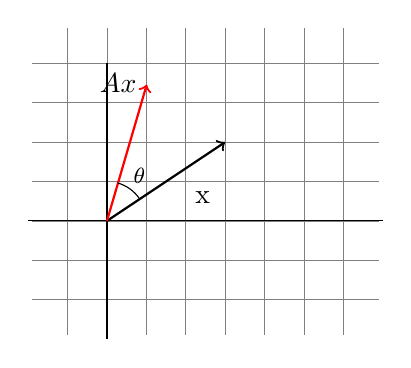
\begin{tikzpicture}[x=0.5cm, y=0.5cm]

\draw[step=0.5cm, style=help lines] (-1.9,-2.9) grid (6.9,4.9);
\draw (-2,0) -- (7,0);
\draw (0,-3) -- (0,4);

\draw[thick,->] (0,0) -- (3,2);
\draw (2,1) node[below right] {\Mtx{x}};

\draw[thick,red,->] (0,0) -- (1.01,3.46);
\draw (1,3) node[above left] {$A\Mtx{x}$};

\draw (0,0) +(34:0.5cm) arc (34:74:0.5cm);
\path (0,0) ++(54:0.7cm) node[font=\footnotesize] {$\theta$};

%\draw (1.5,1) arc (34:74:1cm);
%\path (0,0) ++(55:1.1cm) node[font=\footnotesize] {$\theta$};

\end{tikzpicture}

\end{center}


\end{frame}
%===========================================================


